\section{Measurement}
\label{sec:Durchführung}
For this experiment a Sagnac-Interferometer is chosen because of its high resistance against external disturbances.
\begin{figure}
\centering
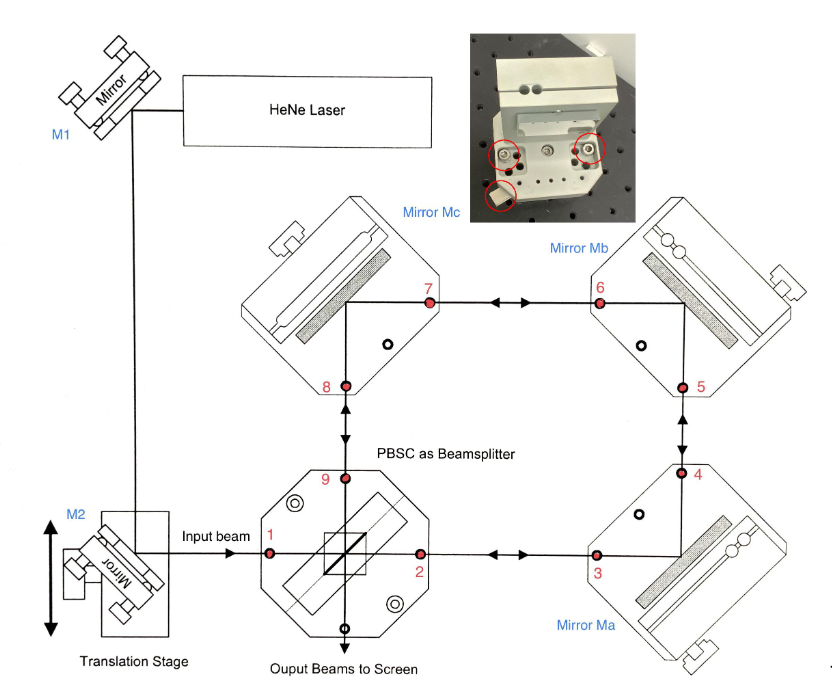
\includegraphics[width=0.8\textwidth]{Sagnac-Interferometer}
\caption{Schematic picture of the Sagnac-Interferometer used for the purpose of this experiment. \cite{V64}}
\label{fig:Sagnac}
\end{figure}
A schematic picture of the interferomter used can be seen in Figure \ref{fig:Sagnac}. The light for the interferometer is generated by a HeNe-Laser emitting linearly polarised light tilted by $45°$ from the vertical with a wavelength of $\SI{632,990}{\nano\meter}$.
\subsection{Adjustment}
To be able to properly use the interferometer for measurements it first has to be adjustet. For this purpose adjustement plates are used to stepwise adjust the interferometer. 

First the mirror $M1$ is adjusted so that the laser beam hits the center of Mirror $M2$. This mirror can then be positioned in a way, that the beam transmitted by the PBSC passes through the center of the adjustment plates in positions $1$ and $2$. Afterwards the reflected beam is adjusted to pass the center of adjustment plates in positions $8$ and $9$ by moving the PBSC itself. Then the mirrors $Ma$ and $MC$ are adjusted using plates in positions $5$ and $6$. In a last step the mirror $Mb$ can be adjusted by using plates in the positions $7$ and $4$. With all adjustement steps finished a polarization filter has to be introduced to the interfering beams to synchronize their polarization angle. The resulting picture should then still show no interference fringes if the interferometer is perferctly adjusted. By moving the mirror $M2$ away from the adjusted central position the two overlapping beams can be separated so that each beam can be manipulated individualy.
\subsection{Measuring the visibility}
To measure the visibility a glass holder with two tilted glass plates at an adjustable angle is introduced to the beam. Each plate has a thickness of $D=\SI{1}{\milli\meter}$. The polarisation angle of the input beam is also additionally controlled by a polarisation filter in front of the PBSC. By utilizing the angle of the glass plates the interference pattern can now be changed to either show a minimum or a maximum. The intensity is measured using the output voltage of a photo-diode. The polarisation of the input beam is then increased in $10°$ steps from $0°$ to $180°$ and for each angle the intensity at the minimum and the maximum are recorded. This measurement is repeated three times.
\subsection{Refractive index of glass}
After the visibility is measured in the previous step the polarisation angle of the input beam is set to guarantee the maximal visibility. For the measurements regarding the refractive indices the difference voltage method is used with two diodes. The angle of the glass plates is then increased from $0°$ to $10°$ and an automatic counter in combination with an oscilloscope is used to measure the number of Maxima. This procedure is repeated ten times.
\subsection{Refractive index of air}
Instead of the glass holder a gas cell with a length of $L=\SI{100\pm0,1}{\milli\meter}$ is then introduced to the beam. The cell can be avacuated using a pump and then slowly filled with air again. The number of Maxima is recorded in steps of $\SI{50}{\milli\bar}$. This measurement is repeated five times.